\chapter{This is the first real chapter}
\graphicspath{{\currfiledir/figures/}}

\lipsum[1]


The well known Pythagorean theorem \(x^2 + y^2 = z^2\) was
proved to be invalid for other exponents.
Meaning the next equation has no integer solutions:

\begin{equation}
	x^n + y^n = z
	.
\end{equation}

\lipsum[2]

\begin{figure}[h]
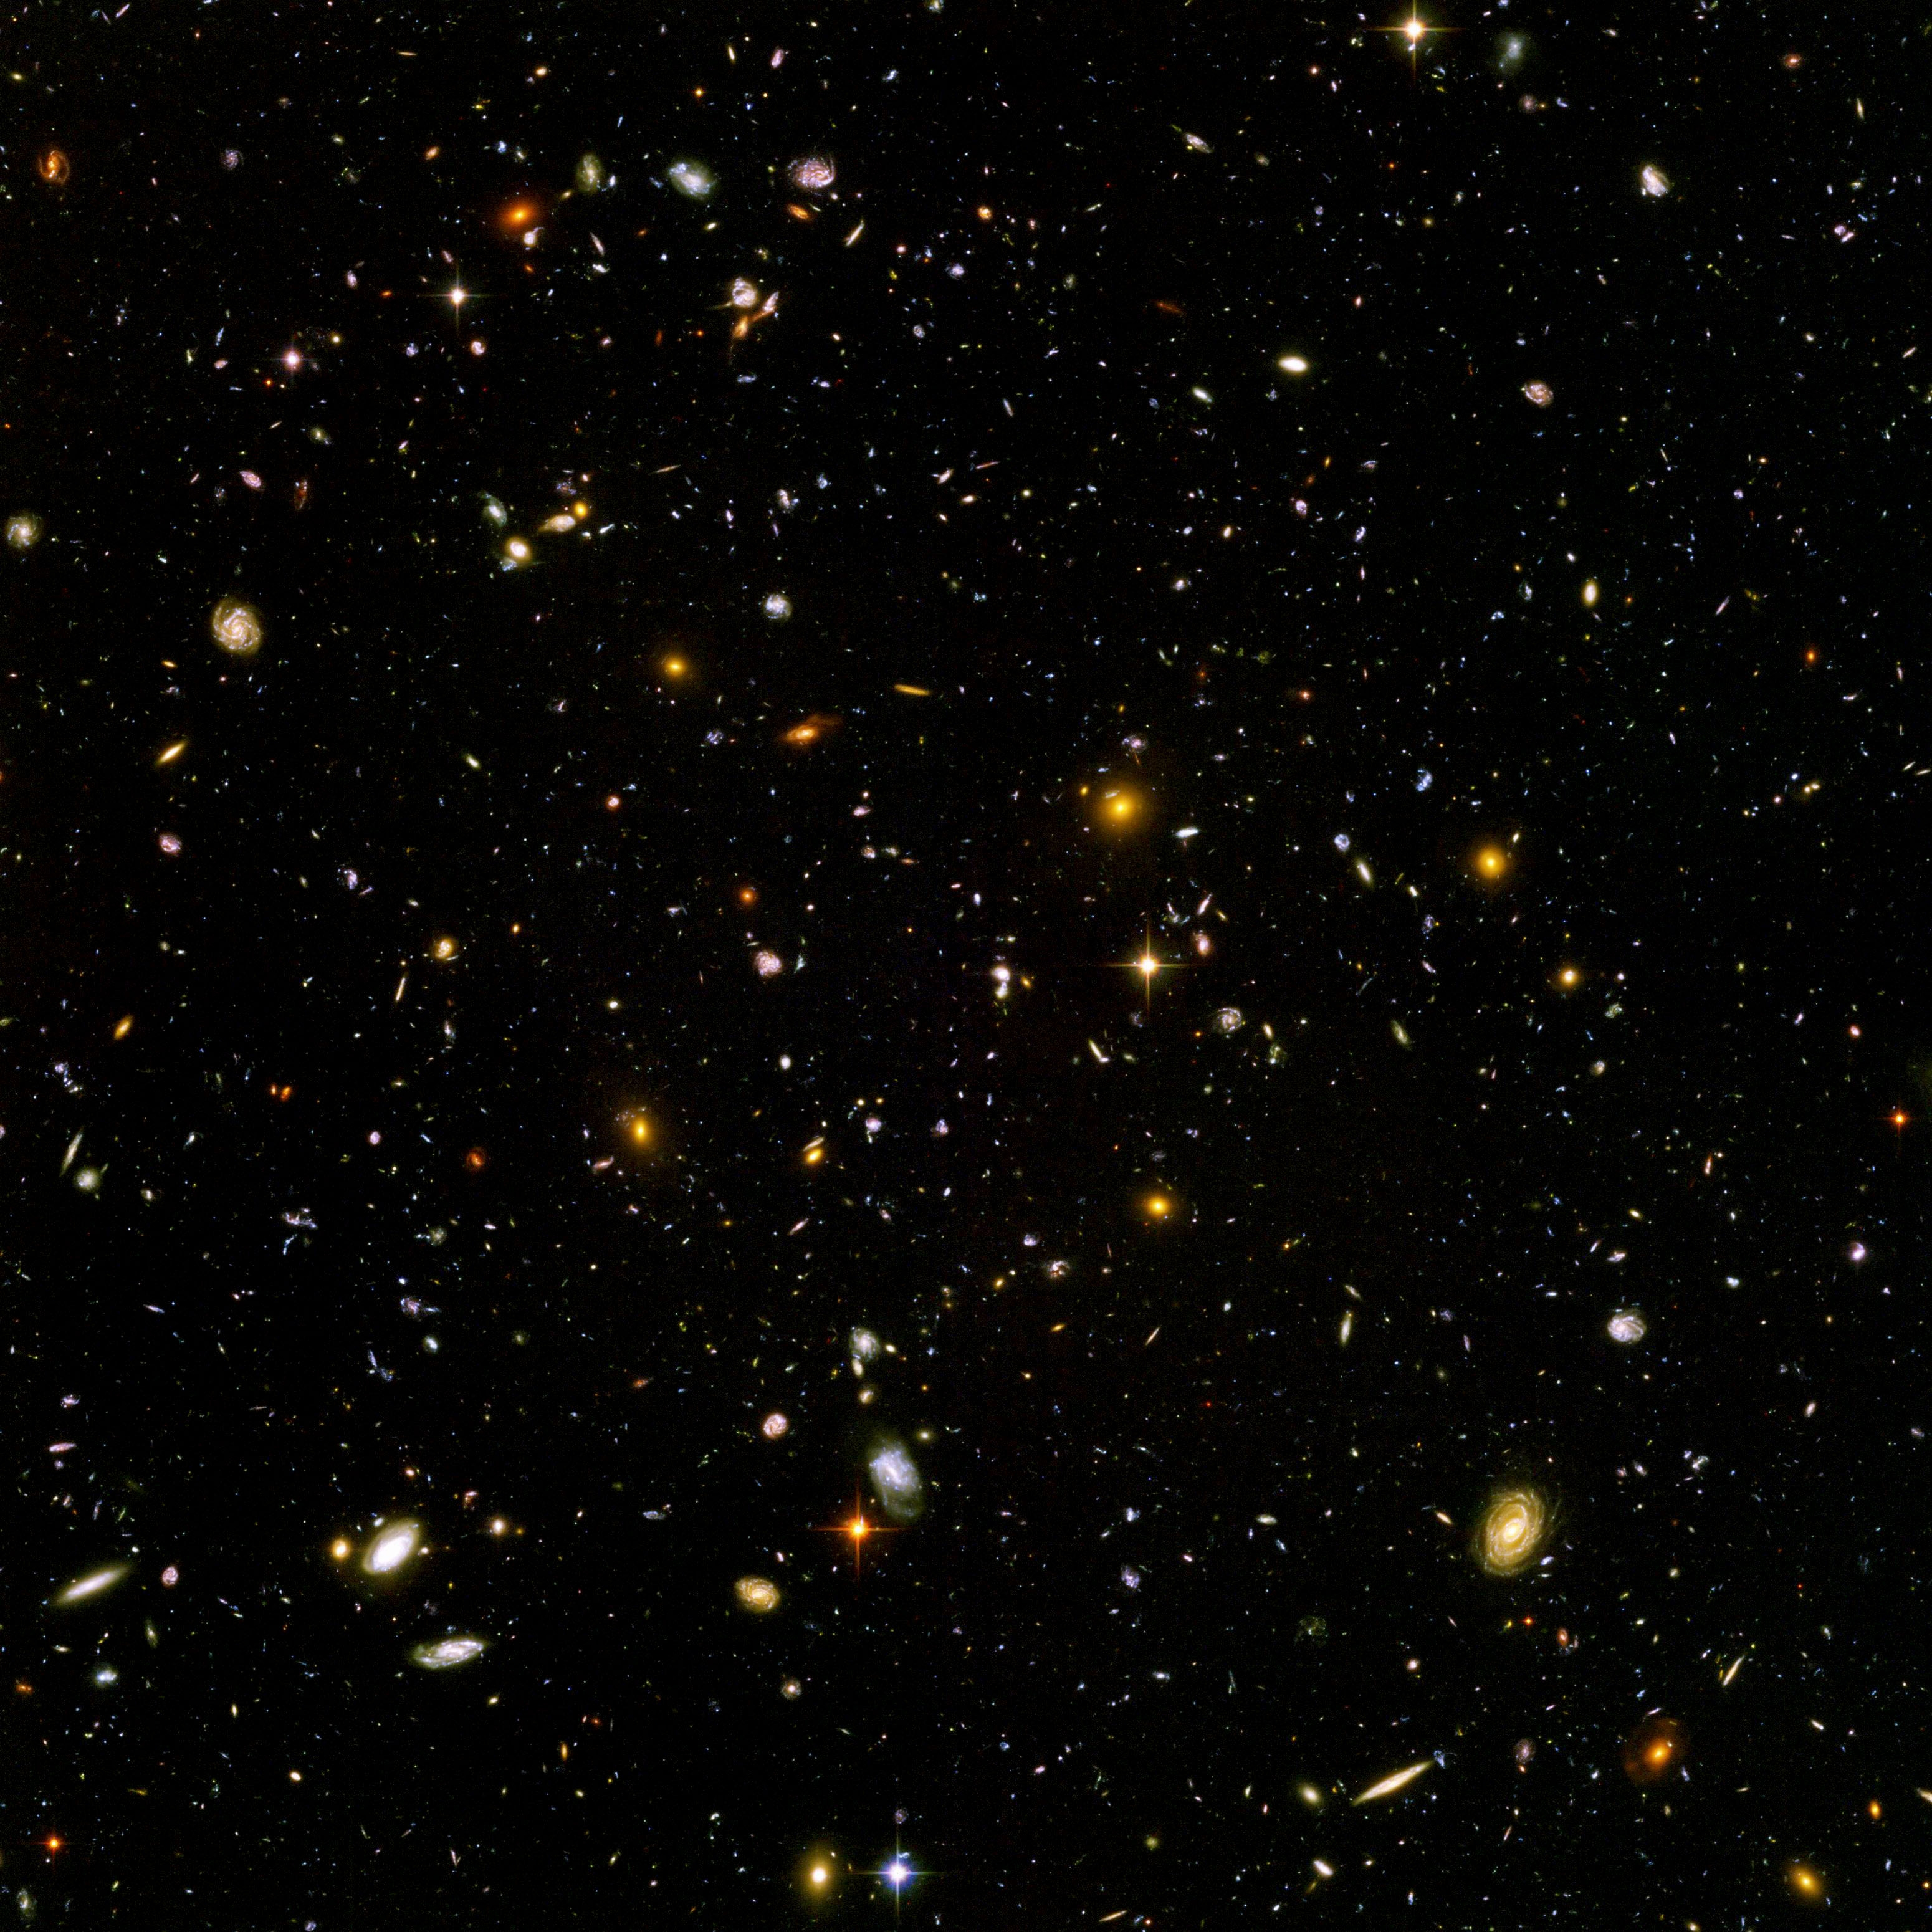
\includegraphics[width=\textwidth]{Hubble_ultra_deep_field.jpg}
\caption{Wikipedia: ``The Hubble Ultra Deep Field, is an image of a small region of space in the constellation Fornax, composited from Hubble Space Telescope data accumulated over a period from September 3, 2003 through January 16, 2004. The patch of sky in which the galaxies reside was chosen because it had a low density of bright stars in the near-field.'' Copyright: NASA and the European Space Agency -- \url{http://hubblesite.org/newscenter/archive/releases/2004/07/image/a/warn/}.}
\label{fig:universe}
\end{figure}

\lipsum[3]

\begin{table}
\centering
\begin{tabular}{ |p{0.22\linewidth}||p{0.22\linewidth}|p{0.22\linewidth}|p{0.22\linewidth}|  }
 \hline
 \multicolumn{4}{|c|}{Country List} \\
 \hline
 Country Name or Area Name& ISO ALPHA 2 Code &ISO ALPHA 3 Code&ISO numeric Code\\
 \hline
 Afghanistan   & AF    &AFG&   004\\
 Aland Islands&   AX  & ALA   &248\\
 Albania &AL & ALB&  008\\
 Algeria    &DZ & DZA&  012\\
 American Samoa&   AS  & ASM&016\\
 Andorra& AD  & AND   &020\\
 Angola& AO  & AGO&024\\
 \hline
\end{tabular}
\caption{This is a random table that I took from the Overleaf examples}
\end{table}

\lipsum[4]


\cite{Langmuir} explains the necessary building blocks for life on any planet.
\bibliographystyle{unsrt}
\bibliography{bibliography}